\problemname{Japanese Lottery}

\illustration{0.32}{japaneselottery}{Strawberry picking game, photo by \href{https://commons.wikimedia.org/wiki/File:\%E3\%82\%A4\%E3\%83\%81\%E3\%82\%B4\%E3\%81\%A4\%E3\%81\%BF\%E3\%82\%B2\%E3\%83\%BC\%E3\%83\%A0\%E3\%81\%A8\%E3\%81\%84\%E3\%81\%86\%E5\%90\%8D\%E3\%81\%AE\%E3\%81\%9F\%E3\%81\%A0\%E3\%81\%AE\%E3\%81\%82\%E3\%81\%BF\%E3\%81\%A0\%E3\%81\%8F\%E3\%81\%98.jpg}{Nanao Wagatsuma}\vspace{-0.5cm}}%
Amida-kuji is a lottery popular in Japan, which can be used to assign~$w$ prizes to~$w$ people.
The game consists of~$w$ vertical lines, called \emph{legs}, and some horizontal bars that connect adjacent legs.
The tops of the legs are the starting positions of the $w$~people, and the prizes are at the bottom of the legs.
To determine the prize of the $i$th person, one has to move down on the $i$th leg, starting at the top, and switch the leg whenever a horizontal bar is encountered.
You can see such a game and how to trace a path in Figure~\ref{fig:amidakuji}.

You want to manipulate the lottery in such a way that the $i$th person gets the $i$th prize,
for every~$i$, by removing some horizontal bars.
Since you do not want to get caught, you want to remove as few bars as possible.

\begin{figure}[h]
	\centering
	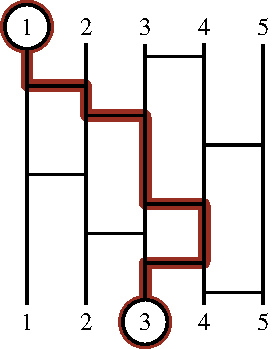
\includegraphics{sample}
	\caption{Visualization of an Amida-kuji game. 
		The first person is connected to the third prize.
		This is also Sample Input 2 after all connections are added and before any connection is removed.
		To connect the $i$th person to the $i$th prize, it suffices to remove both horizontal bars between legs~$2$ and~$3$ and the topmost horizontal bar between legs~$3$ and~$4$.
		This is the only minimal solution.}\label{fig:amidakuji}
\end{figure}

For this problem, the initial game configuration has no horizontal bars.
Then, horizontal bars are added one by one or are removed again.
After each change, you want to know the minimum number of horizontal bars that need to be removed such that the $i$th prize is assigned to the $i$th person for each $i$.
Note that this is always possible by removing all horizontal bars.
	
\vspace{-3mm}
\begin{Input}
	The input consists of:
	\begin{itemize}
		\item One line with three integers $w, h$ and $q$ ($2 \leq w \leq 20$, $1\leq h,q \leq 2\cdot10^5$), the number of legs, the height of the legs, and the number of changes.
		\item $q$ lines, each containing three integers $y, x_{1}$ and $x_{2}$ ($1\leq y \leq h$, $1\leq x_{1}, x_{2} \leq w$), describing a change where a horizontal bar is added or removed at height $y$ between legs $x_1$ and $x_2$.
								If there is already a horizontal bar at this position, it will be removed. Otherwise the bar will be added.
		It is guaranteed that the two legs are adjacent, i.e.\ $|x_{1}-x_{2}|=1$.
	\end{itemize}	
	It is guaranteed that all horizontal bars have different heights at every moment.
\end{Input}

\begin{Output}
	After each change, output a single integer, the minimum number of horizontal bars that need to be
				removed in the game with the currently existing bars such that the $i$th prize is assigned to the $i$th person for each $i$.
\end{Output}
